\documentclass[12pt]{report}
\usepackage[utf8x]{inputenc}
\usepackage[dutch]{babel}
\usepackage{amsmath}
\usepackage{graphicx}
\usepackage{listings}
\usepackage{afterpage}


\lstdefinelanguage{VHDL}{
	morekeywords={
		library,use,all,entity,is,port,in,out,end,architecture,of,
		begin,and, if, else
	},
	morecomment=[l]--
}
\lstset{
	numbers=left,
	breaklines=true,
	tabsize=4,
	literate={\ \ }{{\ }}1
}


\usepackage{xcolor}
\colorlet{keyword}{blue!100!black!80}
\colorlet{comment}{green!90!black!90}

\lstdefinestyle{vhdl}{
	language     = VHDL,
	basicstyle   = \ttfamily,
	keywordstyle = \color{keyword}\bfseries,
	commentstyle = \color{comment}
}

\begin{document}
	\begin{titlepage}
		
		\definecolor{landanimal}{RGB}{00, 66, 121}
		\pagecolor{landanimal}\afterpage{\nopagecolor}
		\center	
		
		\color{white}
		\textsc{\LARGE InHolland}\\[1.5cm] % Name of your university/college
		\textsc{\Large VHDL}\\[2.5cm] % Major heading such as course name
		
		
		\huge \bfseries S88-n Protocol in VHDL \\[2.0cm] % Title of your document
		
		\emph{Authors:}\\
		
		\begin{minipage}{0.4\textwidth}
			\begin{flushleft} \large
				
				Koen Groot \\ nummer
			\end{flushleft}
		\end{minipage}
		~
		\begin{minipage}{0.4\textwidth}
			\begin{flushright} \large
				\large Ruben Pera \\ 551198
			\end{flushright}
		\end{minipage}
	
	
		
	\end{titlepage}
\chapter*{Samenvatting}
Dit verslag gaat over een communicatie kunnen opstellen tussen een NI-FPGA bord en een RM88-N schuifregister via het S88 protocol. Dit wordt tot stand gebracht met de hardware beschrijvingstaal VHDL.\\
Ten eerste wordt onderzocht hoe het S88 protocol werkt. Dit blijkt na extensief onderzoek een protocol te zijn om data over een lijn te sturen. Dit wordt verder gebruikt om data heen weer te sturen vanaf het NI-FPGA bord naar het schuifregister. Er wordt gecontroleerd of het werkt door een LED aan te zetten op het NI-FPGA bord.\\\\

Om te kunnen communiceren is echter wel een constant signaal benodigd, het NI-FPGA bord bevat gelukkig een OnBoardClock (ingebouwde klok) waarmee het mogelijk is te controleren wanneer er een signaal wordt opgevangen.\\
De klok werkt echter op 50Mhz terwijl het RM88-N bord slechts 1khz aankan, dus moet de klok eerst naar beneden geschaalt worden.\\\\

In dit verslag wordt dus besproken wat er geprobeerd wordt te behalen en hoe dit behaald wordt. Met in diepte onderzoek naar de middelen gebruikt. Met name de hardware beschrijvings taal VHDL en het S88 timings protocol.
	\tableofcontents
	\clearpage
	
	\chapter{Inleiding}
	[comments]
	Leg in de inleiding van breed naar smal het probleem in zijn context uit.\\
	Je eindigt de inleiding precies daar waar je het probleem globaal beschreven hebt.\\
	Dan in het hoofdstuk specificatie geef je alle onderdelen weer die door fabrikanten aangeleverd worden, voor zover van toepassing. (Let op! Dit is een keuze, vaak is er een wisselwerkng tussen je specificatie en je requirements en daarmee de volgorde van de hoofdstukken.)\\
	Nu komt de probleem stelling met eventuele onderzoeksvragen aan de orde met daarbij de requirements, etc. Een indeling kun je ook op BB vinden. Die is echter niet zaligmakend,\\ aangezien het kan zijn dat het probleem op zich leidt tot onderzoeksvragen die aanleiding geven tot een hardware keuze.\\
	
	Uiteindelijk moet in je verslag een hoofdstuk het logische vervolg zijn op het vorige hoofdstuk.\\
	

	Geef ter illustratie in dit hoofdstuk ook schematische weergaves van de hardware (het NI-FPGA bord en het RM88-N bord).\\
	Hiernaar kun je dan in je tekst verwijzen.
	
	
	
	
	\chapter{Probleem Omschrijving}
\section{Probleem Omschrijving}

De RM88 is ontworpen om een goedkope feedback bus te zijn, de feedback wordt geleverd via het S88 protocol.\\
Het idee is eenvoudig, de RM88 is een serieel schuif register met een parralelle load input, de input zal dus binnenkomen via het timingsprotocol S88.\\
In dit onderzoek gaat er onderzocht worden of dit nagebouwd kan worden met een XILINX Spartan 3E FPGA bord en de harware omschrijf taal VHDL.


\section{Hoofdvraag}
De Hoofdvraag bij dit onderzoek luidt:
\\\\
Hoe kan er op een XILINX Spartan 3E FPGA bord met behulp van de hardware beschrijving taal VHDL een s88 protocol geïmplementeerd worden?
\\

\section{Deelvragen}
Om de Hoofdvraag goed te kunnen beantwoorden zijn er de volgende deelvragen opgesteld:

\begin{enumerate}
	\item Hoe werkt het s88 protocol?
	\item Hoe werkt een XILINX Spartan 3E FPGA bord?
	\item Hoe kan de hardware beschrijving taal VHDL gebruikt worden op het XILINX bord?
	\item Hoe kan een schuifregister aangesloten worden op het XILINX bord?
\end{enumerate}

Pas nadat alle deelvragen beantwoordt zijn kan op de hoofdvraag een volledig antwoord geformuleerd worden.
	\chapter{Specificaties}
	Bij dit project zijn de volgende drie specificaties meegegeven:
	\begin{enumerate}
		\item Ontwerp en imllementeer een test machine voor de S88.
	\end{enumerate}
	\textit{}\chapter{Vereisten}

Om te kunnen onderzoeken of 

De volgende vereisten zijn gesteld aan het te opleveren systeem.

\begin{itemize}
	\item Het XILINX Spartan 3E FPGA bord moet kunnen communiceren met een Field Programmable Gate Array (FPGA).
	\item De communicatie tussen het XILINX bord en de FPGA moet plaatsvinden door middel van het S88 protocol.
	\item De communicatie tussen het XILINX bord en de FPGA wordt als volgt beschreven, het XILINX bord zal via het S88 protocol de eerste byte uit het FPGA lezen.
	\item Het XILINX bord zal geconfigureerd worden met de hardware beschrijving taal VHDL.
\end{itemize}

	\chapter{Analyse}
In dit onderzoek gaat er onderzocht worden of het S88 protocol nagebouwd kan worden met een XILINX Spartan 3E FPGA bord en de harware omschrijf taal VHDL.
\section{deelvragen}
Voor de Analyse zijn er meerdere deelvragen opgesteld,

\begin{enumerate}
	\item Hoe werkt het s88 protocol?
	\item Hoe werkt een XILINX Spartan 3E FPGA bord?
	\item Hoe kan de hardware beschrijving taal VHDL gebruikt worden op het XILINX bord?
	\item Hoe kan een schuifregister aangesloten worden op het XILINX bord?
\end{enumerate}

\subsection{Hoe werkt het s88 protocol?}
Het s88 wordt uitgelegd met behulp van onderstaande afbeelding.
\\\\
Hierin is CENTRALE het in dit project gebruikte XILINX bord. 
\\\\
Een centrale, die hier CENTRALE heet, kan met behulp van het s88 protocol de rechter bus uitlezen. Dit gebeurt met behulp van een schuifregister.
\\\\
Met de DATA OUT poort van de CENTRALE BUS wordt data ingelezen. Deze is verbonden met de Q1 out poort van het schuifregister, hiermee wordt dus informatie van het schuifregister naar de CENTRALE overgedragen.
\\\\
De werking is als volgt, op het moment dat de CENTRALE een positieve flank geeft op de CLOCK en de LATCH hoog is, dan zal het schuifregister de data op Ingang D inlezen. Geeft de CENTRALE een positieve flank en is de LATCH Laag, dan zal het schuifregister één positie opschuiven.
\\\\
Door een puls op RESET te geven worden de buffers gereset en zijn deze weer gereed voor het ontvangen van nieuwe data. 


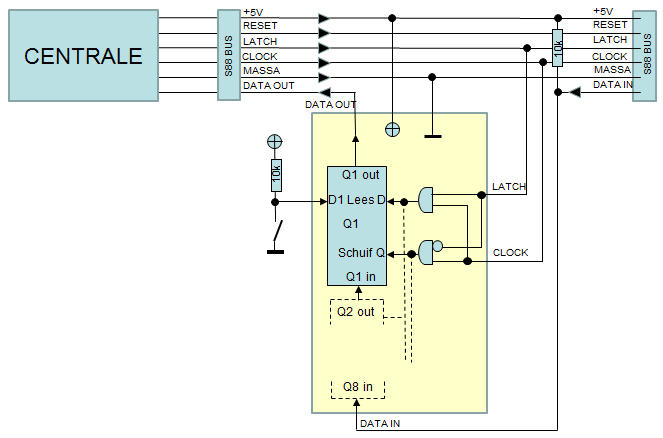
\includegraphics[width=400px]{./img/S88Bus.png}
%http://users.telenet.be/RedDeBist/MBAAN/S88%20terugmelder.htm#S88 bus:
@online{ID,\\
	title = {S88 TERUGMELDERS},\\
	date = {04-03-2016},\\
	url = \url{http://users.telenet.be/RedDeBist/MBAAN/S88\%20terugmelder.htm}
		
	}
\clearpage
	
\subsection{Hoe wordt het XILINX Spartan 3E FPGA bord gebruikt?}
%http://www.xilinx.com/support/documentation/data_sheets/ds312.pdf

\newpage
\subsection{Hoe kan de hardware beschrijving taal VHDL gebruikt worden op het XILINX Spartan 3E FPGA bord?}

%Stuke van Koen

	%\chapter{Ontwerp}
	%\chapter{Implementatie}
	%\chapter{Testen}
	%\chapter{Conclusie}
	%\chapter{Bibliografie}
	
\chapter{Apendix}
	\center

\lstinputlisting[style=VHDL]{./code/works.vhd}

			
\end{document}